\documentclass[10pt]{article}
\usepackage{eecs149}
\usepackage{multicol,caption,url}
\newenvironment{Figure}
  {\par\medskip\noindent\minipage{\linewidth}}
  {\endminipage\par\medskip}
\tikzset{
  >=stealth'
}
\begin{document}
\begin{center}
  \Large Gesture Controlled Driving
\end{center}
\begin{center}
  Ollie Peng, Manish Raghavan, Victor Sutardja
\end{center}
\begin{multicols}{2}
  \section*{Overview}
  Using the Kobuki platform from lab, we built a system by which the Kobuki
  drives in a path drawn by the user. Specifically, the user draws a path in the
  air using a brightly colored object. The Kobuki takes a series of images of
  this path using a webcam mounted on its frame. These images are streamed to a
  laptop which performs the image-processing needed to detect the object used
  for drawing. The points from the images are interpolated into a smooth path.
  Using feedback from the OptiTrack camera system, the Kobuki is instructed to
  drive along this path, correcting for any errors in real time.

  \section*{Setup}
  \begin{Figure}
    \begin{tikzpicture}[->,shorten >=1pt,auto,node distance=2cm, thin]
      \node (m) [rectangle,draw] at (0,0) {Mac};
      \node (k) [rectangle,draw] at (2,0) {Kobuki};
      \node (w) [rectangle,draw] at (-3.5,0) {Windows};
      \node (o) [rectangle,draw] at (-3.5,2) {OptiTrack};

      \path
      (k) edge [bend right=30] node [above] {orientation} (m)
      (m) edge [bend right=30] node [below] {radius and speed} (k)
      (w) edge node [below,align=center] {position and\\orientation} (m)
      (o) edge node [right,align=center] {full tracking\\data} (w)
      ;
    \end{tikzpicture}
    \captionof{figure}{Flow of information} \label{fig:info}
  \end{Figure}

  Figure~\ref{fig:info} shows the flow of information between various devices.
  There are two key design decisions we made in order to overcome challenges we
  faced. First, we streamed the OptiTrack data to a separate Windows machine
  instead of the Mac that was communicating with the data because the frame rate
  from the traking system was too high and would be constantly modifying shared
  variables. Since we were only sending updated commands to the Kobuki once
  every second, we did not need such frequent information, and therefore used
  the Windows machine to sample the data at a lower rate before passing it on
  the Mac. Second, we chose to take orientation data from both the OptiTrack and
  Kobuki. We did so because the orientation from OptiTrack was given in terms of
  quaternions in a rotated axis space, meaning that the standard equations for
  converting to yaw, pitch, and roll no longer applied. Instead, we needed to
  know which quadrant the yaw was in to correct them. As a result, we used the
  orientation from the Kobuki to determine which quadrant it was facing,
  allowing us to use the correct equations to get the true orientation.

  \section*{Image Processing}

  \section*{B-spline Interpolation}
  We chose B-spline interpolation with cubic polynomials because it has the
  following properties: \cite{fuhuacheng2012}
  \begin{itemize}
    \item Locality -- only nearest 3 points affect the curve
    \item Continuity -- continuous up to the second derivative
  \end{itemize}
  B-spline interpolation yields a smooth path, allowing the Kobuki to drive
  without stopping to turn. Intuitively, the interpolation yields a path that is
  at any time a linear combination of three neighboring points, weighted by the
  basis curves at those points. Since the basis curves, shown in
  Figure~\ref{fig:basis} approximate Gaussians when in the middle of the path,
  the interpolation can be viewed as letting each control point have
  ``influence'' on the interpolated curve that depends on how close the curve is
  to that point. However, this means that the interpolated curve does not
  actually pass through the control points. As a result, we had to take in a
  series of data points and find control points such that the resultant curve
  interpolated through the control points passes through the original data
  points. Figure~\ref{fig:sample} shows how from the original data points, shown
  in blue, a series of control points, shown in red, are computed, and when
  interpolated, the final path passes through the data points.

  \begin{Figure}
    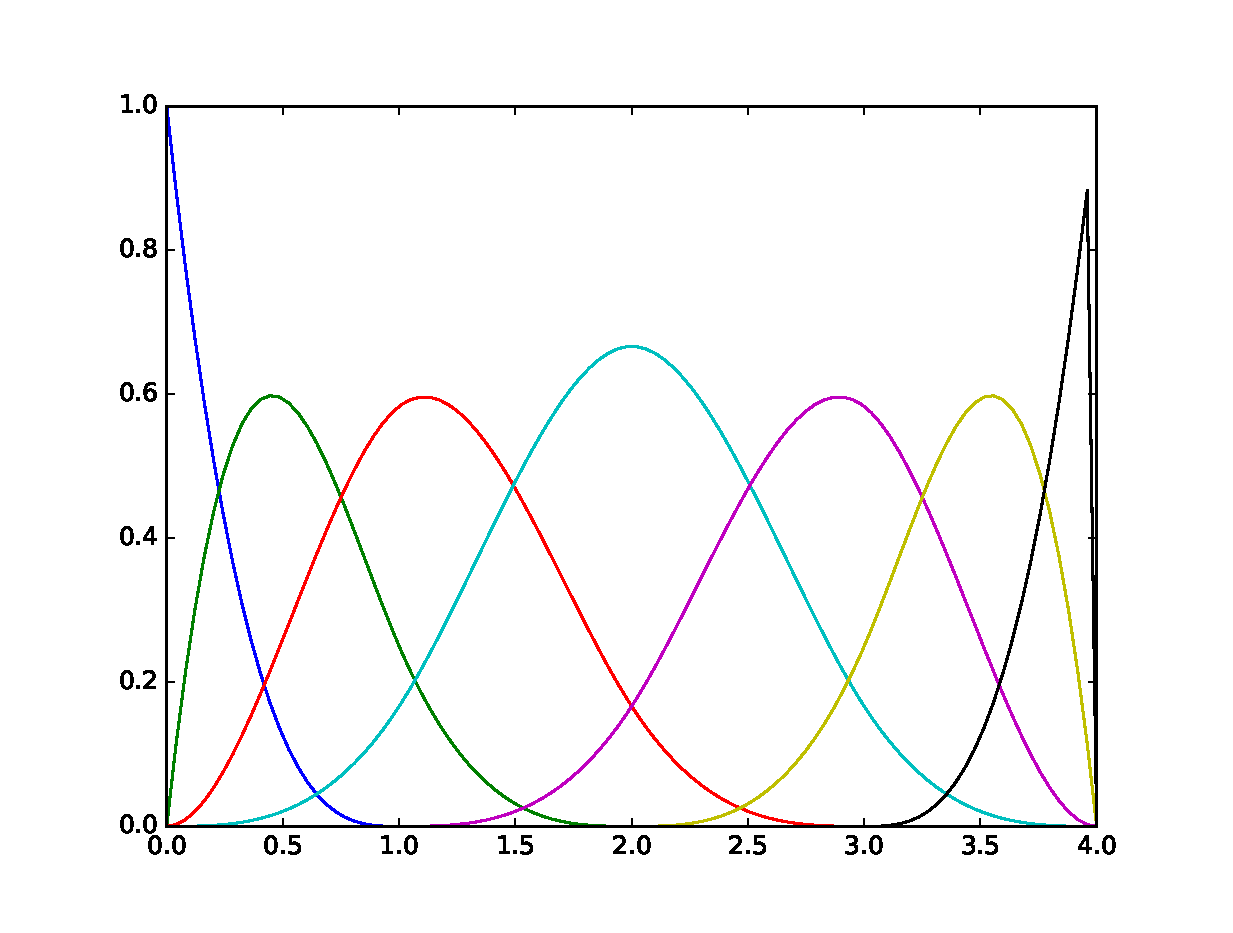
\includegraphics[width=9cm]{../spline_basis.eps}
    \captionof{figure}{Cubic spline basis curves} \label{fig:basis}
  \end{Figure}
  \begin{Figure}
    \includegraphics[width=9cm]{../s_img/spline8.eps}
    \captionof{figure}{Sample cubic spline interpolation} \label{fig:sample}
  \end{Figure}

  By convention, we will assume that we have $n+1$ data points. To ensure that
  the endpoints of the curve are correct, we define \[t_i = \begin{cases}
      0 & 0 \le i \le 3 \\
      i-3 & 3 \le i \le n+3 \\
      n+3 & n+3 \le i \le n+6
    \end{cases}
  \]
  The equations for the basis functions are given by the following recurrence
  relation: \cite{wiki:spline}
  \[N_{i,1}(x) \coloneqq \begin{cases}
      1 &\text{ if } t_i \le x < t_{i+1} \\
      0 &\text{ otherwise}
  \end{cases} \]
  \begin{align*}
    N_{i,k}(x) &\coloneqq \frac{x-t_i}{t_{i+k-1}-t_i} N_{i,k-1}(x) \\
    &+ \frac{t_{i+k}-x}{t_{i+k}-t_{i+1}} N_{i+1,k-1}(x)
  \end{align*}
  In order to get the curve to pass through all the data points, we need 2 more
  control points than data points. To find the control points from the data
  points, we use the fact that the curve must start and end with our first and
  last data points and must pass through each of our data points. Since we have
  $n+3$ control points and $n+1$ data points, we add the initial conditions that
  the second derivative of the curve at the start and end points must be 0. This
  yields the following system of equations:
  \begin{align*}
    \mathbf{P}_0 &= \mathbf{D}_0 \\
    \frac{3}{2} \mathbf{P}_1 - \frac{1}{2} \mathbf{P}_2 &= \mathbf{D}_0 \\
    N_{i,4}(i) \mathbf{P}_i + N_{i+1,4}(i) \mathbf{P}_{i+1} + N_{i+2,4}(i)
    \mathbf{P}_{i+2} &= \mathbf{D}_i \\
    -\frac{1}{2} \mathbf{P}_{n} - \frac{3}{2} \mathbf{P}_{n+1} &= \mathbf{D}_n \\
    \mathbf{P}_{n+2} &= \mathbf{D}_{n}
  \end{align*}
  Solving for these gives us the control points $\mathbf{P}_0, \dots,
  \mathbf{P}_{n+2}$. To interpolate the curve, we simply use
  \[C(t) = \sum_{i=0}^{n+2} N_{i,4}(t) \mathbf{P}_i\]

  \section*{Timing}

  \section*{Threading}
  In controlling the Kobuki, we had to send it instructions while also receiving
  orientation data from it. To do so, we used threading -- one thread listened
  for data from the Kobuki while the other thread used that data to control it.
  In order to prevent race conditions, we used locks on two shared resources:
  the socket over which we were communicating and a global variable containing
  the Kobuki's orientation. Since we had two threads each using the same two
  locks, we had to avoid deadlock, which we did by ensuring that no thread held
  more than one lock at the same time. Each thread executed a task periodically,
  on the order of tenths of a second or longer, meaning that the delay caused by
  waiting for locks was insignificant compared to the running time allowed for
  each task.

  \section*{Modeling Movement and Control}
  \begin{Figure}
    \includegraphics[width=9cm]{../plots/roc.eps}
    \captionof{figure}{Movement planning} \label{fig:roc}
  \end{Figure}

  \section*{Results}
  \begin{Figure}
    \includegraphics[width=9cm]{../plots/s_plot.png}
    \captionof{figure}{Actual vs. planned path} \label{fig:s_plot}
  \end{Figure}
\end{multicols}
\bibliographystyle{plain}
\bibliography{refs}
\end{document}
